% Repository:  https://github.com/chiehrosswang/TRB_LaTeX_tex
%
% Transportation Research Board conference paper template
% version 4.0 Lite (updates made to be compatible in Overleaf and ShareLaTeX)
%
%
% When numbered option is activated, lines are numbered.
\documentclass[numbered]{trbunofficial}
\usepackage{graphicx}
\usepackage{booktabs}

\newread\somefile
\usepackage{xparse}
\usepackage{natbib}
\bibliographystyle{unsrtnat}
\setcitestyle{round}
% \usepackage[colorlinks=true,linkcolor=blue,citecolor=blue]{hyperref}
% For TRB version hide links
\usepackage[hidelinks]{hyperref}

% Put here what will go to headers as author
\AuthorHeaders{Reynolds and Currie}
\title{Benchmarking transit service levels by Local Government Areas
using GTFS feeds}

% TODO: add macros for easier formatting of \author.
\author{%
    \textbf{James Reynolds}\\\textit{Corresponding Author}\\
  Research Fellow\\
  Public Transport Research Group, Institute of Transport Studies,
Department of Civil Engineering, Monash University, Victoria,
Australia\\
  \href{mailto:james.reynolds@monash.edu}{\nolinkurl{james.reynolds@monash.edu}}\\
  \hfill\break
    \textbf{Graham Currie}\\
  Professor\\
  Public Transport Research Group, Institute of Transport Studies,
Department of Civil Engineering, Monash University, Victoria,
Australia\\
  \href{mailto:graham.currie@monash.edu}{\nolinkurl{graham.currie@monash.edu}}\\
  \hfill\break
  }

% If necessary modify the number of words per table or figure default is set to
% 250 words per table (default defined in cls)


% If words are counted manually, put that number here. This does not include
% figures and tables. This can also be used to avoid problems with texcount
% program i.e. if one does not have it installed.
\TotalWords{684}


% tightlist command for lists without linebreak
\providecommand{\tightlist}{%
  \setlength{\itemsep}{0pt}\setlength{\parskip}{0pt}}




\begin{document}
\maketitle


\section{Abstract}
TBC.
\hfill\break%
\hfill\break%
\noindent\textit{Keywords}:  Transit, Public
transport, GTFS, Benchmarking, Local government,  
\newpage

\hypertarget{introduction}{%
\section{Introduction}\label{introduction}}

There are many metrics used to assess and compare transit service
levels. These include those in the Transit Capacity and Quality of
Service Manual (TCQSM) \citep{TCQSM:2013}, which specifies Levels of
Service (LOS) on a scale of A to F across a wide range of measures such
as service span, frequency, speed, proportion of population serviced and
many more. Transit Score instead provides a single rating out of 100,
ranging from ``Rider's Paradise'' for those places scoring above 90, all
the way down to places with a score below 25 where it (may) ``be
possible to get on a bus''\citep{WalkScore:2023tg}.

Practitioners and researchers seeking to use such metrics may face two
inter-related challenges. Firstly, there is the problem of calculating
the metrics themselves for a specific transit system or location.
Secondly, there may be the challenge of explaining the metrics and their
meaning to others, who may not be transit-specialists and might include
politicians, other decision-makers and the general public. The TCQSM and
Transit Score metrics may provide contrasting examples of these
challenges. The TCQSM metrics may be time consuming and challenging to
calculate, given the amount of population, network and other data that
needs to be assembled and included in calculation. Yet,
\citet{TCQSM:2013} provides detailed explanations of how each score is
calculated and what might need to be done to improve service levels.
This set of metrics would appear to be suitable for use amongst
practitioners and researchers, and perhaps in some instances for
interactions with politicians and the general public. However, it may be
challenging to use TCQSM metrics in a press release or for public
advocacy given the level of detail each addresses.

In contract, the Transit Score metric, provides a single and simple
score out of 100, which might be relatively easy to use in public
communications or advocacy. It is also already provided on the
\citet{WalkScore:2023tg} website for locations with a published GTFS
feed, eliminating the need for any calculations. However, the Transit
Score is calculated by a patented algorithm, and so it may not be easy
to understand or explain the connection between real-world conditions
and the score, or what might need to be done to improve the score and
service levels. Nor does it appear to be possible for Transit Scores to
be generated for proposed changes to networks.

Previous research by \citet{Wong:2013aa} overcame some of the
limitations of the TCQSM using Python, PostgreSQL and R software and
GTFS feeds as input. Outputs included daily average headways, route
length and stop numbers, and as the code is opensource this might be
adaptable to further GTFS feeds and purposes. These three metrics may be
particularly useful in communication about the amount of transit service
to a broader audience, as they appear relatively simple to understand.
However, they are route based, and so do not include any consideration
of geographic or population coverage.

\citet{currie2007identifying} developed a Supply Index, representing the
amount of transit supplied for a Census Collection District (CCD) of
interest. This takes into account service coverage through the inclusion
of a buffer zone around each stop to account for typical walk access
distances to stops. This index appears to have the advantage of being
relatively easy to calculate, and easy to explain and understand.
However, as yet this measure has not been calculated directly from GTFS
data.

This paper reports research undertaken to fill this gap by developing R
code to calculate the Supply Index of \citet{currie2007identifying}
directly from GTFS data. The code is developed using data from a single
case: the GTFS for Victoria in Australia, which includes Greater
Melbourne. Cross-case comparison to Toronto, Canada, and Washington DC,
USA, is also undertaken to test the results and gain understanding of
how the Supply Index might be useful for practitioners, researchers and
advocates. The motivation for this research is to better understand how
transit service levels and changes might benchmarked for non-technical
audiences.

\hypertarget{research-context}{%
\section{Research context}\label{research-context}}

\hypertarget{general-transit-feed-specification-gtfs}{%
\subsection{General Transit Feed Specification
(GTFS)}\label{general-transit-feed-specification-gtfs}}

\hypertarget{social-needs-and-the-suppy-index}{%
\subsection{Social needs and the Suppy
Index}\label{social-needs-and-the-suppy-index}}

\footnote{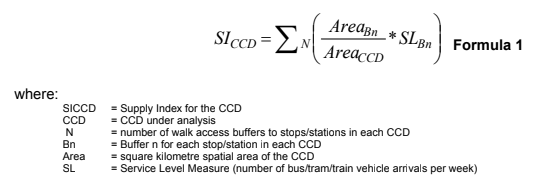
\includegraphics{Supply_index.png}}

he SI\textsubscript{CCD} can then be compared between different CCDs to
give an indication of the relative supply of transit, adjusted for
accessibility.

An advantage of the Supply Index is that it is a relatively simple
number to calculate, understand and explain. It is based on the number
of bus/tram/train arrivals per week at stops within the CCD, which is
multiplied by a factor allowing for the amount of the CCD that is within
walking distance of each stop \footnote{This is the
  Area\textsubscript{Bn} divided by Area\textsubscript{CCD} part of the
  calculation. Thresholds for access of 400m for bus and tram stops, and
  800m for railway stations are used in the calculation of the
  Area\textsubscript{Bn} variable.}.

\citet{currie2007identifying} calculated the SI for various CCDs in
Melbourne using a timetable database provided by the Victorian Public
Transport Authority (PTA). This predated the widespread availability of
GTFS data, which provides a standardised format for timetable data that
is produced by many transit systems. A question, therefore, is how to
calculate the SI using GTFS data so that SI\textsubscript{CCD}s can be
calculated for current services in Melbourne or other places.

\hypertarget{methodology}{%
\section{Methodology}\label{methodology}}

\hypertarget{results}{%
\section{Results}\label{results}}

\hypertarget{discussion}{%
\section{Discussion}\label{discussion}}

\hypertarget{conclusions}{%
\section{Conclusions}\label{conclusions}}

\hypertarget{author-contribution-statement}{%
\section{Author Contribution
Statement}\label{author-contribution-statement}}

The authors confirm contribution to the paper as follows: study
conception and design: A. Anonymous, D. Zoolander; data collection: B.
Security; analysis and interpretation of results: A. Anonymous, B.
Security; draft manuscript preparation: A. Anonymous. All authors
reviewed the results and approved the final version of the manuscript.

\hypertarget{acknowledgements}{%
\section{Acknowledgements}\label{acknowledgements}}

This document was prepared using the \texttt{rticles} template, created
by Gregory Macfarlane, which is based on the \LaTeX originally posted by
David Pritchard in 2009 and updated it in 2011, soon after TRB began
allowing PDF submissions. Gregory Macfarlane and Ross Wang made
adjustments to the template, and Ross Wang now maintains the
\LaTeX template at \url{https://github.com/chiehrosswang/TRB_LaTeX_tex}.
Gregory Macfarlane created the \texttt{rticles} template in 2021.

\newpage
\renewcommand\refname{References}
\bibliography{packages.bib,benchmarkingLGAGTFS.bib}


\end{document}
